\chapter{Current Intensity and the Ammeter}\label{ch:g8:intensity-ammeter}

``Strong current, weak current'' --- we have talked this way for
years, dosing brightness and grip by feel. Feel retires today.
The current's strength gets a name, a \omterm{def:g6:measurement-in-science:measuring}{unit} and an instrument;
and the first thing the instrument proves is a law you have
long suspected but never once measured.

\section{Intensity and its unit}

\begin{definition}[Intensity]\label{def:g8:intensity-ammeter:intensity}
The \emph{intensity}\index{intensity} $I$ of an \omterm{def:g7:circuits-series-parallel:current}{electric current}
\omterm{def:g6:measurement-in-science:measuring}{measures} how strong the march is: how much electric charge
parades past a point of the circuit each second --- the
current's flow rate, as a river's is water-per-second. Its \omterm{def:g6:measurement-in-science:measuring}{unit}
is the \emph{ampere}\index{ampere} (\unit{A}), honoring a great
pioneer of electricity's laws; everyday circuits often speak in
\emph{milliamperes}: $\qty{1}{mA} = \qty{0.001}{A}$, a
thousandth.
\end{definition}

\begin{example}[Amperes to know by sight]\label{ex:g8:intensity-ammeter:values}
A little indicator lamp sips about \qty{0.02}{A} ---
\qty{20}{mA}; a flashlight \omterm{def:g3:first-electric-circuit:bulb}{bulb}, around \qty{0.3}{A}; the great
lamp of a car's headlight, \qty{5}{A}; a kettle at full roar,
\qty{10}{A}; a starting car engine gulps \qty{100}{A} from its
\omterm{def:g3:first-electric-circuit:battery}{battery}; a lightning stroke, for its millisecond, rams tens of
thousands of \omterm{def:g8:intensity-ammeter:intensity}{amperes} down its channel. And the danger scale is
sobering: currents of a few hundredths of an \omterm{def:g8:intensity-ammeter:intensity}{ampere} across a
human body can already be fatal --- respect begins well below
one \omterm{def:g8:intensity-ammeter:intensity}{ampere}.
\end{example}

\begin{remark}[The person and the unit]\label{rem:g8:intensity-ammeter:person}
Written out, the \omterm{def:g6:measurement-in-science:measuring}{unit} is lowercase --- ``a current of two
\omterm{def:g8:intensity-ammeter:intensity}{amperes}'' --- while the capitalized word names the person, as
with every \omterm{def:g6:measurement-in-science:measuring}{unit} honoring a scientist. The symbol \unit{A} stays
capital. You will meet this convention again shortly, twice.
\end{remark}

\section{The ammeter}

\begin{definition}[Ammeter]\label{def:g8:intensity-ammeter:ammeter}
An \emph{ammeter}\index{ammeter} \omterm{def:g6:measurement-in-science:measuring}{measures} \omterm{def:g8:intensity-ammeter:intensity}{intensity}. It counts
the march that passes \emph{through itself} --- so it must be
inserted \emph{\omterm{def:g4:series-circuits:series}{in series}}, into the very loop it \omterm{def:g6:measurement-in-science:measuring}{measures}, like
a tollbooth on the road. Built to disturb the march as little
as possible, it opposes the current almost not at all --- which
is also why an ammeter misconnected straight across a \omterm{def:g3:first-electric-circuit:battery}{battery}
is a \omterm{def:g7:short-circuits-safety:device}{short circuit} with a dial: the classic way to break one.
\end{definition}

\begin{method}[Measuring an intensity]\label{met:g8:intensity-ammeter:measure}
\begin{enumerate}
  \item switch the circuit off; \emph{break} the loop where the
        current is to be counted;
  \item insert the \omterm{def:g8:intensity-ammeter:ammeter}{ammeter} into the gap: current in by its
        \unit{A} \omterm{def:g3:first-electric-circuit:battery}{terminal}, out by its \emph{common} \omterm{def:g3:first-electric-circuit:battery}{terminal},
        so the conventional direction enters the meter's front
        door;
  \item on a multi-range meter, start on the \emph{largest}
        range, then step down until the reading sits
        comfortably on the dial --- protecting the meter from
        surprises;
  \item close the \omterm{ex:g3:first-electric-circuit:switch}{switch}, read --- and write the \omterm{def:g6:measurement-in-science:measuring}{unit}.
\end{enumerate}
Backward connection on a needle meter slams the needle against
its stop; digital meters merely show a minus sign, forgiving
students daily.
\end{method}

\begin{omfigure}
\begin{tikzpicture}[scale=0.9]
  \draw (0,0) to[battery1, l=battery] (0,2.8)
    to[short] (1.8,2.8)
    to[ammeter, l=$I$] (4.2,2.8)
    to[lamp, l=lamp] (6.6,2.8)
    to[short] (8.0,2.8)
    to[short] (8.0,0)
    to[short] (0,0);
  \draw[-Stealth, very thick, omThm] (1.0,3.15) -- (1.7,3.15);
\end{tikzpicture}

{\small The \omterm{def:g8:intensity-ammeter:ammeter}{ammeter} takes its place in the loop: a tollbooth \omterm{def:g4:series-circuits:series}{in
series}, counting the march that \omterm{def:g1:light-and-shadows:source}{lights} the lamp.}
\end{omfigure}

\begin{omfigure}
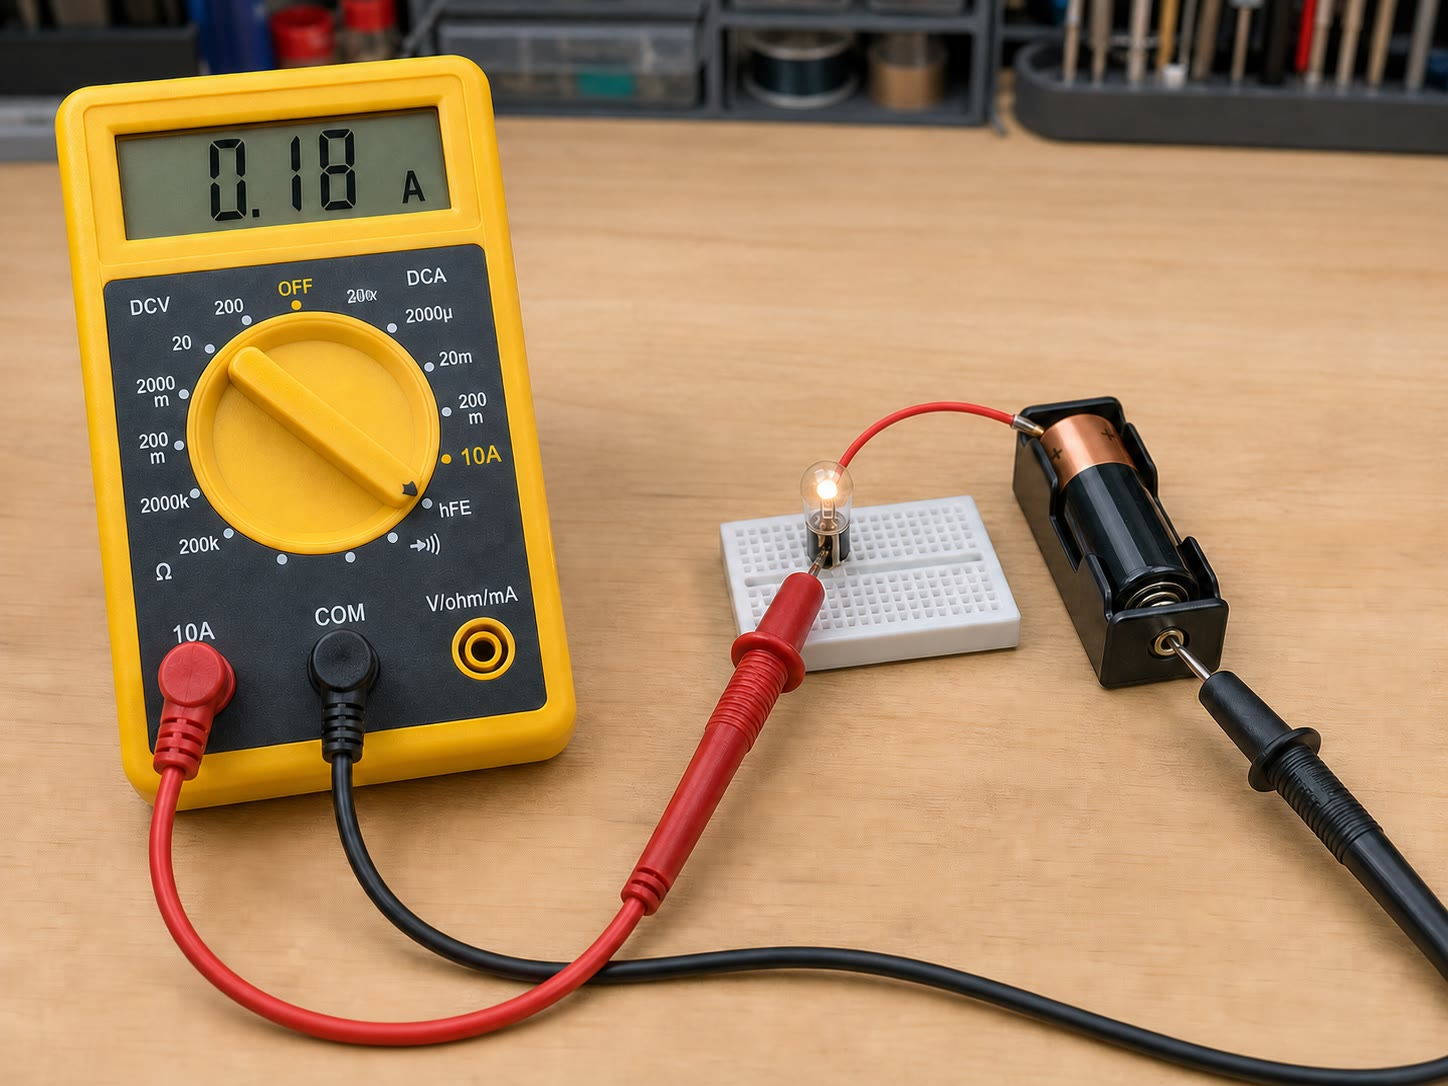
\includegraphics[width=0.5\linewidth]{images/book1/ai/g8-ammeter-multimeter.jpg}

{\small The workbench reality: one instrument, two probes, and the circuit's current becomes a number on the display.}
\end{omfigure}

\section{The first measured law}

\begin{proposition}[One loop, one intensity]\label{prop:g8:intensity-ammeter:sameI}
In a \omterm{def:g4:series-circuits:series}{series circuit}, the \omterm{def:g8:intensity-ammeter:intensity}{intensity} is the same at every point of
the loop. Move the \omterm{def:g8:intensity-ammeter:ammeter}{ammeter} anywhere --- before the lamp, after
it, beside the \omterm{def:g3:first-electric-circuit:battery}{battery}: the reading does not change. What five
years of equal-brightness \omterm{def:g3:first-electric-circuit:bulb}{bulbs} suggested, the meter now states
in numbers: nothing is consumed en route; one road, one march,
one $I$.
\end{proposition}

\begin{omfigure}
\begin{tikzpicture}[scale=0.85]
  \draw (0,0) to[battery1] (0,3.0)
    to[ammeter, l=\qty{0.30}{A}] (2.6,3.0)
    to[lamp] (4.8,3.0)
    to[ammeter, l=\qty{0.30}{A}] (7.4,3.0)
    to[lamp] (9.6,3.0)
    to[short] (9.6,0)
    to[ammeter, l=\qty{0.30}{A}] (4.8,0)
    to[short] (0,0);
\end{tikzpicture}

{\small Three tollbooths on one loop: before, between and after
the lamps, every \omterm{def:g8:intensity-ammeter:ammeter}{ammeter} reports the same \qty{0.30}{A}.}
\end{omfigure}

\begin{example}[Reading the law's fine print]\label{ex:g8:intensity-ammeter:fineprint}
The law says \emph{along one loop}, not \emph{whatever you do to
the loop}. Add a second lamp \omterm{def:g4:series-circuits:series}{in series} and the march weakens
everywhere at once --- perhaps \qty{0.30}{A} drops to
\qty{0.17}{A} --- but it weakens \emph{equally} everywhere: the
three tollbooths agree on the new number too. One loop, one
\omterm{def:g8:intensity-ammeter:intensity}{intensity} --- whatever that \omterm{def:g8:intensity-ammeter:intensity}{intensity} currently is.
\end{example}

\begin{example}[A glance at the junction]\label{ex:g8:intensity-ammeter:junction}
Set tollbooths on a parallel pair instead: main road
\qty{0.50}{A}; \omterm{def:g5:series-parallel-circuits:parallel}{branch} one \qty{0.30}{A}; \omterm{def:g5:series-parallel-circuits:parallel}{branch} two
\qty{0.20}{A}. The suggestive sum is no accident --- the marches
into a \omterm{def:g5:series-parallel-circuits:parallel}{junction} and out of it must balance, since charge is
neither created nor destroyed at a fork in the road. The full
law, with its partner for voltage, holds court in the
chapter after next; your meters have already met it.
\end{example}

\begin{remark}[The multimeter]\label{rem:g8:intensity-ammeter:multimeter}
The workshop's yellow brick --- the \emph{multimeter} --- folds
the \omterm{def:g8:intensity-ammeter:ammeter}{ammeter} and several other instruments into one box with a
selector dial. Dial on \unit{A} or \unit{mA}, leads in the
marked sockets, and it is your \omterm{def:g8:intensity-ammeter:ammeter}{ammeter}, series rules and all.
Two chapters of this book live inside it already; a third moves
in next chapter --- with, beware, \emph{opposite} wiring rules.
\end{remark}

\section{Exercises}

\begin{exercise}[$\star$]\label{exo:g8:intensity-ammeter:1}
What does \omterm{def:g8:intensity-ammeter:intensity}{intensity} \omterm{def:g6:measurement-in-science:measuring}{measure}, in river-language? Give its \omterm{def:g6:measurement-in-science:measuring}{unit}
and symbol, and convert \qty{250}{mA} to \omterm{def:g8:intensity-ammeter:intensity}{amperes}.
\end{exercise}

\begin{exercise}[$\star$]\label{exo:g8:intensity-ammeter:2}
Match the \omterm{def:g8:intensity-ammeter:intensity}{intensity} to its scene: \qty{0.02}{A}; \
\qty{0.3}{A}; \ \qty{10}{A}; \ \qty{100}{A} --- kettle,
indicator lamp, starting engine, flashlight \omterm{def:g3:first-electric-circuit:bulb}{bulb}.
\end{exercise}

\begin{exercise}[$\star$]\label{exo:g8:intensity-ammeter:3}
Why must an \omterm{def:g8:intensity-ammeter:ammeter}{ammeter} be inserted \omterm{def:g4:series-circuits:series}{in series}? What is it built to
oppose almost not at all, and what accident does that make
possible?
\end{exercise}

\begin{exercise}[$\star$]\label{exo:g8:intensity-ammeter:4}
List the four steps of a proper \omterm{def:g8:intensity-ammeter:intensity}{intensity} measurement. Why
start on the largest range?
\end{exercise}

\begin{exercise}[$\star$]\label{exo:g8:intensity-ammeter:5}
State the one-loop-one-intensity law. Which old
equal-brightness observation did it turn into numbers?
\end{exercise}

\begin{exercise}[$\star$]\label{exo:g8:intensity-ammeter:6}
An \omterm{def:g8:intensity-ammeter:ammeter}{ammeter} before a series \omterm{ex:g6:circuits-and-safety:motor}{motor} reads \qty{0.45}{A}. What will
it read after the \omterm{ex:g6:circuits-and-safety:motor}{motor}? And beside the \omterm{def:g3:first-electric-circuit:battery}{battery}?
\end{exercise}

\begin{exercise}[$\star$]\label{exo:g8:intensity-ammeter:7}
A second lamp joins a series loop and the \omterm{def:g8:intensity-ammeter:ammeter}{ammeter}'s
\qty{0.30}{A} becomes \qty{0.17}{A}. Has the law failed?
Explain the fine print.
\end{exercise}

\begin{exercise}[$\star$]\label{exo:g8:intensity-ammeter:8}
A digital \omterm{def:g8:intensity-ammeter:ammeter}{ammeter} reads $-0.25$ \unit{A}. What has the student
done, and how grave is it?
\end{exercise}

\begin{exercise}[$\star\star$]\label{exo:g8:intensity-ammeter:9}
Main road \qty{0.60}{A}; \omterm{def:g5:series-parallel-circuits:parallel}{branch} one \qty{0.35}{A}. What does
\omterm{def:g5:series-parallel-circuits:parallel}{branch} two carry, and by what reasoning? What does the second
\omterm{def:g5:series-parallel-circuits:parallel}{junction}'s tollbooth read?
\end{exercise}

\begin{exercise}[$\star\star$]\label{exo:g8:intensity-ammeter:10}
A student wires the \omterm{def:g8:intensity-ammeter:ammeter}{ammeter} \emph{\omterm{def:g5:series-parallel-circuits:parallel}{in parallel}} with the lamp
``to compare them''. Predict the two consequences --- for the
lamp, and for the meter --- and name the villain the student
has accidentally built.
\end{exercise}

\begin{exercise}[$\star\star$]\label{exo:g8:intensity-ammeter:11}
Two identical \omterm{def:g3:first-electric-circuit:bulb}{bulbs} \omterm{def:g5:series-parallel-circuits:parallel}{in parallel} each carry \qty{0.30}{A}. The
\omterm{def:g7:short-circuits-safety:battery}{battery's} main road carries how much? A third identical \omterm{def:g3:first-electric-circuit:bulb}{bulb}
joins \omterm{def:g5:series-parallel-circuits:parallel}{in parallel}: predict the main road's new burden, and
name what drains faster.
\end{exercise}

\begin{exercise}[$\star\star\star$]\label{exo:g8:intensity-ammeter:12}
Design the full measurement plan for a \omterm{def:g5:series-parallel-circuits:parallel}{two-branch} \omterm{def:g5:series-parallel-circuits:parallel}{parallel
circuit} (lamp and \omterm{ex:g6:circuits-and-safety:motor}{motor}): how many \omterm{def:g8:intensity-ammeter:ammeter}{ammeter} positions are
needed to know \emph{every} current in the circuit; the
minimum number of measurements that suffices (one may be
deduced --- by which balance?); and the order of operations
that never leaves a meter wired dangerously.
\end{exercise}

\section{Problem: The Metrology Bench}

\begin{problem}[{Weekend problem --- qualifying day at the
electronics workshop; four stations, one ammeter each; the
apprentice's license}]\label{pb:g8:intensity-ammeter:1}
To earn workshop privileges, each apprentice tours four
measurement stations. Bring the chapter.

\medskip\noindent\textbf{Part I --- Station one: the simple
loop.}
\omterm{def:g3:first-electric-circuit:battery}{Battery}, \omterm{ex:g3:first-electric-circuit:switch}{switch}, one lamp.
\begin{enumerate}
  \item Describe, step by step, inserting the \omterm{def:g8:intensity-ammeter:ammeter}{ammeter} to
        \omterm{def:g6:measurement-in-science:measuring}{measure} the lamp's current.
  \item The reading: \qty{280}{mA}. Express it in \omterm{def:g8:intensity-ammeter:intensity}{amperes}.
  \item The examiner moves your meter to the \omterm{def:g7:short-circuits-safety:battery}{battery's} other
        side. Predict the reading, citing the law.
  \item ``And if I had two \omterm{def:g8:intensity-ammeter:ammeter}{ammeters} in this loop at once?''
        Where could they sit, and what would they show?
\end{enumerate}

\medskip\noindent\textbf{Part II --- Station two: series
pair.}
Two different lamps, A brighter than B, \omterm{def:g4:series-circuits:series}{in series}.
\begin{enumerate}[resume]
  \item An apprentice predicts: ``Brighter A carries more
        current than dim B.'' Test the prediction with the law
        --- and reconcile the equal currents with the unequal
        brightness (what must differ between the lamps?).
  \item The meter reads \qty{150}{mA} between A and B. Write
        down every other current in the loop.
  \item Lamp B is \omterm{def:g7:short-circuits-safety:device}{short-circuited} by a clip lead. Predict the
        new reading and both lamps' behavior.
  \item The examiner asks for one sentence on why the workshop
        forbids clip leads across the \emph{\omterm{def:g3:first-electric-circuit:battery}{battery}} while
        permitting the demonstration across B.
\end{enumerate}

\medskip\noindent\textbf{Part III --- Station three: the
\omterm{def:g5:series-parallel-circuits:parallel}{junction}.}
A lamp \omterm{def:g5:series-parallel-circuits:parallel}{branch} and a \omterm{ex:g6:circuits-and-safety:motor}{motor} \omterm{def:g5:series-parallel-circuits:parallel}{branch} \omterm{def:g5:series-parallel-circuits:parallel}{in parallel}.
\begin{enumerate}[resume]
  \item Main road: \qty{0.52}{A}; lamp \omterm{def:g5:series-parallel-circuits:parallel}{branch}: \qty{0.30}{A}.
        The \omterm{ex:g6:circuits-and-safety:motor}{motor} \omterm{def:g5:series-parallel-circuits:parallel}{branch}'s current, by balance?
  \item The \omterm{ex:g6:circuits-and-safety:motor}{motor} jams (still connected, not turning) and its
        \omterm{def:g5:series-parallel-circuits:parallel}{branch} climbs to \qty{0.40}{A}. Assuming the lamp
        \omterm{def:g5:series-parallel-circuits:parallel}{branch} keeps its \qty{0.30}{A}, what does the main
        road carry now --- and which workshop guard is
        listening?
  \item The lamp is unscrewed. Predict all three tollbooth
        readings.
  \item Why does the \omterm{def:g3:first-electric-circuit:battery}{battery} drain fastest with both \omterm{def:g5:series-parallel-circuits:parallel}{branches}
        healthy --- where is generosity paid?
\end{enumerate}

\medskip\noindent\textbf{Part IV --- The license.}
\begin{enumerate}[resume]
  \item Write the apprentice's pledge: three lines --- where an
        \omterm{def:g8:intensity-ammeter:ammeter}{ammeter} belongs and never belongs; what one loop
        guarantees; what a \omterm{def:g5:series-parallel-circuits:parallel}{junction} balances.
\end{enumerate}
\end{problem}
